\section{Software Architecture}\label{software_architecture}

\begin{figure}[h]
       \centering
       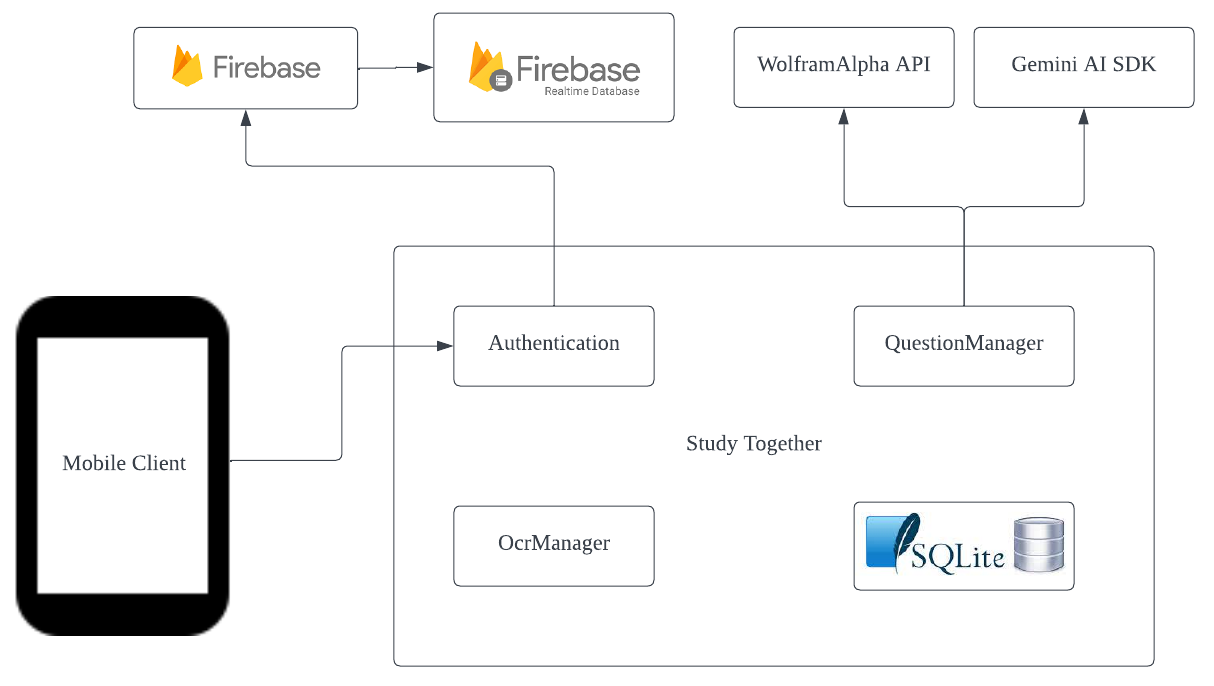
\includegraphics[width=\textwidth]{Figures/StudyTogether_Architecture.png}
       \caption{\footnotesize Initial Software Architecture}
       \label{StudyTogether_Architecture}
\end{figure}

% The software architecture of our Android application, "Study Together," is depicted in the diagram. Our application makes extensive use of Firebase SDK for Authentication and Database services. Additionally, it employs a SQLite database to create and manage a local cache derived from Firebase Database, thereby enhancing overall performance. Data caching occurs immediately after user login, with user data stored in the Room database to eliminate the need for repeated logins. Upon user logout, the database is cleared.

% At the heart of our application lies the QuestionManager Package, which serves as the cornerstone for managing questions and answers. This module seamlessly integrates with Google's Gemini AI API and WolframAlpha API to provide users with potential answers to their queries. Furthermore, it offers functionalities for users to upload and vote on recommended answers.

% Moreover, our application features an OcrManager component equipped with an Optical Character Recognition (OCR) library. This component enables the extraction of text or questions from images captured by the device's camera, streamlining the process of uploading questions for users.

% Our Real-time Chat leverages on the Firebase Database as well, providing users with seamless communication and collaboration features within the application.


% need someone to read thru this again, I modded it and added on notification stuff inside alr - Jovian %
Our Android application "Study Together" harnesses a robust software architecture that leverages Firebase SDK for secure authentication and real-time database interactions. A SQLite database is employed to manage a local cache, which synergizes with the Firebase Database to boost app performance. This local caching is particularly efficient as it retains user data in the Room database post-login, reducing the need for frequent authentication and thus streamlining the user experience. Upon logout, the cache is responsibly cleared to maintain privacy and device performance.

Central to "Study Together" is the QuestionManager Package, a comprehensive module designed for handling the core functionality of questions and answers within the app. It interfaces with Google's Gemini AI API and WolframAlpha API, providing users with intelligent and automated potential solutions. Additionally, this package allows users to contribute by uploading their own answers and participating in a communal voting system to surface the most helpful responses.

% Enhancing user interaction with the app, the OcrManager component incorporates an OCR library, enabling users to easily convert images into text. This feature simplifies the process of question submission, as users can quickly extract text from pictures taken with their device cameras, thereby facilitating a hassle-free question upload experience.
The OcrManager is implemented as an individual activity, designed to be deployed in multiple places as needed. The activity, using a view model, typically uses the live data holding an UI state class, to switch between different composable screens swiftly. Different features are developed as sub-components in the activity, such as download manager, image-saving manager, and the text recogniser. This modular design allows the components of the activity be easily reused.

Complementing these features is the app's Real-time Chat function, also powered by Firebase Database, which offers a seamless platform for users to engage in discussions and collaborate in real-time.

Integrating with this architecture, our notification system is designed to enhance user engagement without compromising the simplicity of the user interface. By providing daily notifications for new questions from followed accounts, we maintain an informative yet unobtrusive service. The notifications are succinct, including the poster's profile image, name, and question topic, and are delivered in accordance with user permissions set in the app, emphasizing our commitment to user control and privacy. This feature is an extension of our user-centric design philosophy, ensuring that "Study Together" not only facilitates academic collaboration but also respects the preferences and autonomy of its user base.
 

\subsection{Application Architecture}\label{application_architecture}

Our application architecture aligns with the classic Model-View-ViewModel (MVVM) design pattern, emphasizing the separation of concerns to ensure modularity. In adherence to this approach, we have distinct \texttt{data} classes separated from the \texttt{view}, with the \texttt{ViewModel} responsible for managing view states. This architectural choice enhances maintainability and scalability.

Moreover, we leverage the Android Application Lifecycle to streamline our notification service. A pivotal aspect of our architecture is the adoption of the Android Application architecture, which advocates for the segregation of the UI Layer from the Data Layer. To achieve this, we employ \texttt{Repositories} to facilitate data modification through Service Calls, while leveraging Data Access Objects (\texttt{DAO}) or \texttt{Retrofit} for interfacing with Firebase, RoomDB or Online APIs like WolframAlpha, depending on the data storage and retrieval requirements.

The rationale behind adopting this architecture lies in its potential for scalability and the clear separation of concerns it offers. By adhering to this approach, different segments of the application can seamlessly implement the Service \texttt{Interface}, enabling the provision of alternative storage backends, thus ensuring flexibility and adaptability.

